\documentclass{report}
\usepackage{listings}
\usepackage{xcolor}
\lstset { %
    language=C++,
    backgroundcolor=\color{black!5}, % set backgroundcolor
    basicstyle=\footnotesize,% basic font setting
    breaklines
}
\usepackage{graphicx}
\usepackage{url}
\usepackage{hyperref}
\hypersetup{
    colorlinks=true,
    linkcolor=blue,
    filecolor=magenta,      
    urlcolor=cyan,
}


\title{Development of the Planes Game, a Version of the Battleships Game}
\date{2017-06-09}
\author{Cristian Cucu}
\begin{document}
\maketitle
\newpage
\lstset{language=C++}
\tableofcontents{}

\chapter{Introduction}

\section{Game Description}
The game is a variant of the classical \href{https://en.wikipedia.org/wiki/Battleship_(game)}{battleship game}. The ships will be here called planes and are shown in \ref{fig:board}.
\begin{figure}[h]
  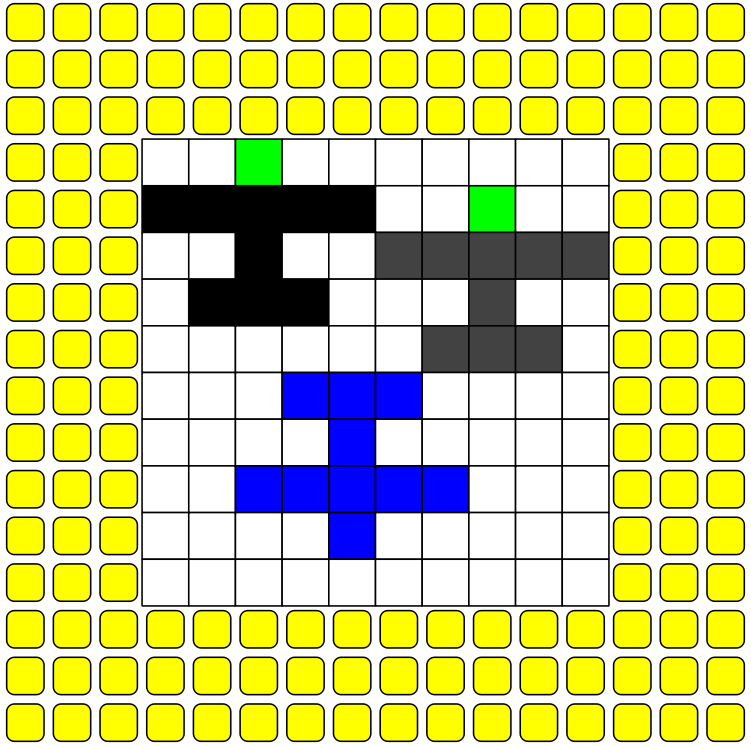
\includegraphics[width = \textwidth]{BoardWithPlanes.png}
  \caption{Board game with 3 planes}
  \label{fig:board}
\end{figure}
The project is organized in two main parts: the game engine and the graphical user interfaces. The game engine is meant to be implemented as a library such it can be used with a number of graphical frontents. One of the design goals is to make this engine independent of a specific C++ library. Three Graphical User Interfaces (GUI) based on the Qt framework were programmed up to this point. They are called PlanesWidget, a simple QWidget approach which also includes debugging tools for the computer's strategy, PlanesGraphicsScene, a GUI based on the QGraphicsScene API, and PlanesQML, based on the QML engine. Another graphical user interface was programmed with Java and interfaces through the Java Native Interface to the C++ game engine.

The complete source code of the projects can be found in GitHub (\url{https://github.com/xxxcucus/planes}).

\chapter {The Game Engine }
\section{Requirements Analysis}
We need an object that describes a plane which should at least contain information about the position of the plane on the game grid, the orientation of the plane, the shape of a plane. Additionaly we would need a game board/grid object. It should not be restricted to a specific geometry, should know where each plane is positioned and how many planes there are. Since the game is played against the computer there should be a kind of strategy object that decides the computer's next move. The organization of the game into a series of human vs. computer rounds needs also to be modelled in code.

\section{The Plane Object}
A plane object is defined through the position of its head  (plane front) and its orientation (see \ref{fig:plane_orientations}).  We assume that each plane exists somewhere in its own reference system and in its own rectangular grid - that is a plane object is not explicitly related to a game board object. 

\begin{figure}[h]
  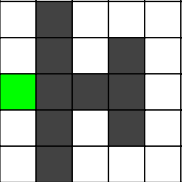
\includegraphics[width = 3cm]{PlaneEastWest.png}
  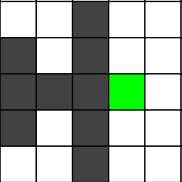
\includegraphics[width = 3cm]{PlaneWestEast.png}
  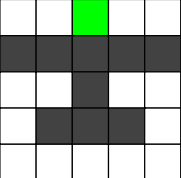
\includegraphics[width = 3cm]{PlaneNorthSouth.png}
  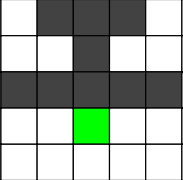
\includegraphics[width = 3cm]{PlaneSouthNorth.png}
  \caption{Possible plane orientations}
  \label{fig:plane_orientations}
\end{figure}

\subsection{Class declaration}
\begin{lstlisting}[caption = {Plane Class Declaration},label=plane_declaration]
class Plane
{
public:
    enum Orientation { NorthSouth = 0, SouthNorth = 1, WestEast = 2, EastWest = 3 };

private:
    //plane orientation
    Orientation m_orient;
    //coordinates of the position of the head of the plane
    int m_row, m_col;

public:
    //Various constructors
    Plane();
    Plane(int row, int col, Orientation orient);
    Plane(const PlanesCommonTools::Coordinate2D& qp, Orientation orient);

    //setter and getters
    //gives the planes orientation
    Orientation orientation() const {return m_orient; }
    //gives the plane head's row and column
    int row() const { return m_row; }
    int col() const { return m_col;}
    //sets the plane head position
    void row(int row) { m_row = row; }
    void col(int col) { m_col = col; }
    void orientation(Orientation orient) { m_orient = orient; }
    //gives the coordinates of the plane head
    PlanesCommonTools::Coordinate2D head() const { return PlanesCommonTools::Coordinate2D(m_row, m_col); }

    //operators
    //compares two planes
    bool operator==(const Plane& pl1) const;
    //translates a plane by a 2d translation vector
    Plane operator+(const PlanesCommonTools::Coordinate2D& qp);

    //geometrical transformations
    //clockwise rotation of planes
    void rotate();
    //translation with given offset in a grid with row and col rows and columns
    //if the future head position is not valid do not translate
    void translateWhenHeadPosValid(int offsetX, int offsetY, int row, int col);

    //other utility functions
    //tests whether a point is a plane's head
    bool isHead(const PlanesCommonTools::Coordinate2D& qp) const { return qp == head(); }
    //checks if a certain point on the grid is on the plane
    bool containsPoint(const PlanesCommonTools::Coordinate2D& qp) const;
    //returns whether a plane position is valid (the plane is completely contained inside the grid) in a grid with row and col
    bool isPositionValid(int row, int col) const;
    //generates a random number from 0 and valmax-1
    static int generateRandomNumber(int valmax);
    //displays the plane
    std::string toString() const;
};
\end{lstlisting} 

\subsection {Method Implementation}
\begin{lstlisting}[caption = {Plane Class Methods}, label=plane_implementation]
//Various constructors
Plane::Plane() {
    m_row = 0;
    m_col = 0;
    m_orient = NorthSouth;
}

Plane::Plane(int row, int col, Orientation orient) {
    m_row = row;
    m_col = col;
    m_orient = orient;
}

Plane::Plane(const PlanesCommonTools::Coordinate2D& qp, Orientation orient) {
    m_row = qp.x();
    m_col = qp.y();
    m_orient = orient;
}

//equality operator
bool Plane::operator==(const Plane& pl1) const {
    return ((pl1.m_row == m_row) && (pl1.m_col == m_col) && (pl1.m_orient == m_orient));
}

//Clockwise 90 degrees rotation of the plane
void Plane::rotate() {
    switch(m_orient)
    {
    case NorthSouth:
        m_orient = EastWest;
        break;
    case EastWest:
        m_orient = SouthNorth;
        break;
    case SouthNorth:
        m_orient = WestEast;
        break;
    case WestEast:
        m_orient = NorthSouth;
        break;
    default:
        return;
    }
}

//checks to see if a plane contains a certain point
//uses a PlanePointIterator which enumerates
//all the points on the plane
bool Plane::containsPoint(const PlanesCommonTools::Coordinate2D& qp) const {
    PlanePointIterator ppi(*this);

    while(ppi.hasNext())
    {
        PlanesCommonTools::Coordinate2D qp1 = ppi.next();
        if(qp == qp1)
            return true;
    }

    return false;
}

//Checks to see if the plane is
//in its totality inside a grid
//of size row X col
bool Plane::isPositionValid(int row, int col) const {
    PlanePointIterator ppi(*this);

    while(ppi.hasNext())
    {
        PlanesCommonTools::Coordinate2D qp = ppi.next();
        if(qp.x()<0 || qp.x()>=row)
            return false;
        if(qp.y()<0 || qp.y()>=col)
            return false;
    }

    return true;
}

//utility function
//generates a random number
int Plane::generateRandomNumber(int valmax) {
    double rnd = rand()/ static_cast<double>(RAND_MAX);
    if (rnd==1.0)
        rnd = 0.5;
    int val = static_cast<double>(valmax)*rnd;

    return val;
}

//constructs a string representation of a plane
//used for debugging purposes
std::string Plane::toString() const
{
    std::string toReturn = "";

    toReturn = toReturn + "Plane head: ";
    toReturn = toReturn + std::to_string(m_row);
    toReturn = toReturn + "-";
    toReturn = toReturn + std::to_string(m_col);
    toReturn = toReturn + " oriented: ";

    switch(m_orient)
    {
    case NorthSouth:
        toReturn = toReturn + "NorthSouth";
        break;
    case SouthNorth:
        toReturn = toReturn + "SouthNorth";
        break;
    case EastWest:
        toReturn = toReturn + "EastWest";
        break;
    case WestEast:
        toReturn = toReturn + "WestEast";
        break;
    default:
        ;
    }

    return toReturn;
}

void Plane::translateWhenHeadPosValid(int offsetX, int offsetY, int row, int col) {
    if ((m_row + offsetX < 0) || (m_row + offsetX >= row)) {
        return;
    }

    if ((m_col + offsetY < 0) || (m_col + offsetY >= col)) {
        return;
    }

    m_row += offsetX;
    m_col += offsetY;
}

//implements plane translation
Plane Plane::operator+(const PlanesCommonTools::Coordinate2D& qp) {
    return Plane(this->m_row + qp.x(), this->m_col + qp.y(), this->m_orient);
}
\end{lstlisting}

The implementation of the member functions of the class Plane is trivial. One thing requires an explanation : the class PlanePointIterator. It has to do with the fact that it exists nowhere in the Plane class definition an explicit representation of the points of the game board corresponding to the plane, in other words of the form of a plane. The only things that are defined are the point of origin or the head as well as the orientation of the plane. Thus the class is general allowing the use of any plane form as long as a plane head and orientation are given. In order to allow to work with the plane's form the class PlanePointIterator is used. It encapsulates the form of the plane but also gives a method to \textit iterate on the grid positions corresponding to the plane. 

\subsection {C++ Concepts}

\subsubsection {Class Definition}
Classes are the building blocks of C++ programs. They define properties of program objects as well as operations that can be performed on or with them. A class definition is a program block:
\begin{lstlisting}
class {
.......
};
\end{lstlisting}
Between the two parantheses  are included member variable declarations and method declarations. 

\subsubsection {Member Variable Declaration}
When object is seen as a box with pieces the member variables are the denomination of the placeholders for the pieces. The values of the member variables can be thought as descriptions of the object's state. Each member variable declaration consist of a type name and a variable name. The type name corresponds to the type of the variable, for example simple types as int, char, double or class types.
The listing below shows the member variable declarations in the Plane class.
\begin{lstlisting}
class {
    Orientation m_orient;
    int m_row, m_col;
};
\end{lstlisting}

\subsubsection {Class Method Declaration}
The methods of a class are declared in the corpus of the class and are analogous to function declarations in C: in their simple form they consist of a return type followed by a function name which is followed by function parameters listed in paranthesis after the function name.

\subsubsection {Setters and Getters}
Setters and getters are methods of a class that either change or read a member variable's value. Normally the member variables are not directly visible to the user of an object, but only through the means of class methods of which the simplest are the getters and the setters.
\begin{lstlisting}
    int row() const { return m_row; }
    int col() const { return m_col;}
    void row(int row) { m_row = row; }
    void col(int col) { m_col = col; }
\end{lstlisting}

\subsubsection {Constructor definition}
Constructors of a class are functions that are always called when the object is created. One of their task is the initialization of the member variables.
\begin{lstlisting}
    Plane();
    Plane(int row, int col, Orientation orient);
    Plane(const PlanesCommonTools::Coordinate2D& qp, Orientation orient);
\end{lstlisting}
In the Plane class declaration we declare three constructors. The declaration is similar to a class method declaration except for they have no return types. The three constructors initialize the three member variables of the class Plane with the data that they receive as parameters. 

\subsubsection {Static methods}
Class methods are called with an object of their associated class. Static class methods do not require an object of the associated class. The Plane class has only one such method which generates a random number.
\begin{lstlisting}
static int generateRandomNumber(int valmax);
\end{lstlisting}

\subsubsection {Enums}

\begin{lstlisting}
    enum Orientation {NorthSouth=0, SouthNorth=1, WestEast=2, EastWest=3};
\end{lstlisting}
Enums are basic types for which the variable values are listed at the time of type definition. In our case the new type is called Orientation and variables of this type can have the following values: NorthSouth, SouthNorth, WestEast, EastWest. For enums the associated variable values can be explicitly converted to int. As shown in the example above the conversion to int can be specified directly in the enum definition. Sometimes one desires to avoid such a conversion and to enforce a strict type checking when assigning enum variables to values. In this case one should use the 'enum class' instead of the simple enum.  

\subsubsection {Access Specifiers}
Elements of classes (methods or member variables) can have specified different levels of access to the class user. These are 
\begin{itemize}
\item public, the element is accessible from all functions
\item private, the element is accessible only from the class methods
\item protected, the element is accessible from the class methods or from derived class methods
\end{itemize}  
In the code above the member variables have private access specifiers and such they are not accessible directly from functions other than the class methods. However setter and getter functions are defined with public acces in order to allow access to these members from everywhere in the program. 

\subsubsection {Operators}
Operators such as
\begin{lstlisting}
    bool operator==(const Plane& pl1) const;
    Plane operator+(const PlanesCommonTools::Coordinate2D& qp);
\end{lstlisting}
are syntactic sugar meant to simplify coding. For example, when defining \textit{operator==} one can directly write the comparison \textit{ plane1 == plane2 } with the meaning of a test of equality (if the operator definition respects the semantics of an identity test). 

\subsubsection {What is '*this' ? }
The function containsPoint(..) uses the operator '*this' with the meaning of the object calling the function. More exactly the constructor of the PlanePointIterator object with the name ppi receives as parameter the object on which the containsPoint() function is called.

\begin{lstlisting}
bool Plane::containsPoint(const PlanesCommonTools::Coordinate2D& qp) const {
    PlanePointIterator ppi(*this);

    while(ppi.hasNext())
    {
        PlanesCommonTools::Coordinate2D qp1 = ppi.next();
        if(qp == qp1)
            return true;
    }

    return false;
}
\end{lstlisting}

\subsubsection {Function parameters and their transmission}

An important problem in a C++ program is how the parameters are transmitted (or passed) to functions. There are three important situations: transmission by value, transmission by reference, transmission by const reference.  

When we have a function which has as parameters of simple types (int, double, char, bool) we normally use parameter transmission by value, like in the example below. In passing by value copies of the parameters will be made and the copies will be used by the function. That means that, on one hand, any change that these parameters undergo in function code will not be perceived by the caller of the function, but, on the other hand, a copy operation is involved which for complex data types can be costly.

\begin{lstlisting}
void Plane::translateWhenHeadPosValid(int offsetX, int offsetY, int row, int col) {
    if ((m_row + offsetX < 0) || (m_row + offsetX >= row)) {
        return;
    }

    if ((m_col + offsetY < 0) || (m_col + offsetY >= col)) {
        return;
    }

    m_row += offsetX;
    m_col += offsetY;
}
\end{lstlisting}

For complexer function parameters we want to avoid the copying associated to the passing of the parameters and hence use references types for the parameters. As an example we examine the function containsPoint() from the Plane class:

\begin{lstlisting}
//checks to see if a plane contains a certain point
//uses a PlanePointIterator which enumerates
//all the points on the plane
bool Plane::containsPoint(const PlanesCommonTools::Coordinate2D& qp) const {
    PlanePointIterator ppi(*this);

    while(ppi.hasNext())
    {
        PlanesCommonTools::Coordinate2D qp1 = ppi.next();
        if(qp == qp1)
            return true;
    }

    return false;
}
\end{lstlisting}

The parameter of the function which is of the type PlanesCommonTools::Coordinate2D is passed as a reference, that is a reference to it is given to the function. No copying is involved. Had it not been for the const keyword before the qp parameter the function containsPoint could have modified the value of the parameter in the caller's scope (at the caller). In fact this is a method used to return parameters calculated in functions to the function caller (e.g. when more than one parameters need to be returned by a function). In our concrete case the parameter qp is declared const (see also \ref {Constness}) and the compiler will forbid calling non-const operations on it. Passing parameters as const references is the most employed method of parameter passing as it avoids a copy operation and forbids the changing of the parameter at the caller.  
\section{PlanePointIterator Class}

The PlanePointIterator is responsible with enumerating the points of a plane object and is very often used in other source files. The following section describes the design of this class.

\subsection {Class declaration}

\begin{lstlisting}
//iterates over the points that make a plane
class PlanePointIterator : public ListIterator<QPoint>
{
    Plane m_plane;
public:
    PlanePointIterator(const Plane& pl);

private:
    void generateList();
};
\end{lstlisting}

The definition above says that the PlanePointIterator is defined as a type of ListIterator \textless QPoint \textgreater which is defined (here I anticipate the ListIterator class definition which is given later) as an iterator over a list of QPoint objects. It receives a Plane object with which it generates, with the help of the private function generateList, the list of positions occupied by the plane on the game board. It is a type of Java-like iterator, but this will become apparent only after looking at the ListIterator class. 

\subsection {Method implementation}
\begin{lstlisting}
//constructor
PlanePointIterator::PlanePointIterator(const Plane& pl):
    MyIterator::ListIterator<QPoint>(),
    m_plane(pl)
{
    generateList();
}

//the function that generates the list of points
void PlanePointIterator::generateList()
{
    const QPoint pointsNorthSouth[] = {QPoint(0, 0), QPoint(0, 1), QPoint(-1, 1), QPoint(1, 1), QPoint(-2, 1), QPoint(2, 1), QPoint(0, 2),
                                   QPoint(0, 3), QPoint(-1, 3), QPoint(1, 3)};

    const QPoint pointsSouthNorth[] = {QPoint(0, 0), QPoint(0, -1), QPoint(-1, -1), QPoint(1, -1), QPoint(-2, -1), QPoint(2, -1), QPoint(0, -2),
                                   QPoint(0, -3), QPoint(-1, -3), QPoint(1, -3)};

    const QPoint pointsEastWest[] = {QPoint(0, 0), QPoint(1, 0), QPoint(1, -1), QPoint(1, 1), QPoint(1, -2), QPoint(1, 2), QPoint(2, 0),
                                 QPoint(3, 0), QPoint(3, -1), QPoint(3, 1)};

    const QPoint pointsWestEast[] = {QPoint(0, 0), QPoint(-1, 0), QPoint(-1, -1), QPoint(-1, 1), QPoint(-1, -2), QPoint(-1, 2), QPoint(-2, 0),
                                 QPoint(-3, 0), QPoint(-3, 1), QPoint(-3, -1)};

    const int size = 10;
    for(int i = 0;i < size; ++i)
    {
        switch(m_plane.orientation())
        {
            case Plane::NorthSouth:
                m_internalList << pointsNorthSouth[i] + m_plane.head();
                break;
            case Plane::SouthNorth:
                m_internalList << pointsSouthNorth[i] + m_plane.head();
                break;
            case Plane::WestEast:
                m_internalList << pointsWestEast[i] + m_plane.head();
                break;
            case Plane::EastWest:
                m_internalList << pointsEastWest[i] + m_plane.head();
                break;
            default:
                ;
        }
    }
}

\end{lstlisting}

PlanePointIterator is an iterator that provides access to the positions occupied by the plane on the game board. Its constructor receives as Parameter an object of the class Plane, which defines the position of the plane's head as well as its orientation. The method generateList() contains the positions of cells belonging to a plane relative to the position of its head for each of the four possible plane orientations. To calculate the positions of the cells corresponding to the plane it chooses the right set of relative positions according to the given plane orientation and then it adds them to the absolute position of the plane head.

To create a game with other forms of ships it is sufficient to reimplement the PlanePointIterator class.

\subsection {Implementation of ListIterator}

The essence of a PlanePointIterator is captured by the ListIterator class : a PlanePointIterator is a method (defined in the ListIterator class) to iterate over a list together with a special list, defined with the method generateList().

\begin{lstlisting}
namespace MyIterator
{
//defines an iterator over a QList
template <class T>
class ListIterator
{
protected:
    QList <T> m_internalList;
    int m_idx;

public:
    //constructor
    ListIterator();

    //sets the position of the iterator before the first  element
    void reset();
    //during an iteration checks to see if there is a next element
    bool hasNext() const;
    //during an iteration returns the next element
    const T& next();
    //returns number of elements
    int itemNo() const;
};

template <class T>
ListIterator<T>::ListIterator()
{
    //generates the list of points
    m_internalList.clear();
    //puts the index one before the first element in the list
    reset();

}

template <class T>
void ListIterator<T>::reset()
{
    m_idx = -1;
}

//during a point iteration checks to see if there is a next point
template <class T>
bool ListIterator<T>::hasNext() const
{

    return (m_idx<m_internalList.size()-1);
}

//during an iteration returns the next point
template <class T>
const T& ListIterator<T>::next()
{
    return  m_internalList[++m_idx];
}

//returns number of points on the plane
template <class T>
int ListIterator<T>::itemNo() const
{
    return m_internalList.size();
}
}
\end{lstlisting}

ListIterator is a parametrizable class (a so called template class) which has only two member variable, a list (implemented through the Qt type QList) and an index inside the list. 

\subsection {C++ Concepts}
\subsubsection {Iterators}

Iterators are methods to obtain sequential access to the members of a data container (e.g. vector, list, set). No assumption about the order in which the data is retrieved should be made. In the simplest application scenario an iterator is initialized, an action is performed to the data pointed by the iterator, then the iterator is incremented to the next position and so further until the end of data structure is reached. For a C++ style iterator this would look like this:

\begin{lstlisting}
	//initialization of the iterator at the beginning
	auto it = storage.begin();    
	// read data as long as the data end has not been encountered	
	while (it != storage.end()) {  
		//do something with the data pointed to by the iterator		
		do_something(*it);   
		//go to the next position in the data storage 
   		++it;   
	}
\end{lstlisting}

For a Java style iterator this would be:

\begin{lstlisting}
	//initialize iterator with data	
	auto it(storage);     
	//as long as data is available    
	while (it.hasNext()) { 
		//read the data and jump to the next value
		auto d = it.next();  
		//do something with the data
        do_something(d);  
    }
\end{lstlisting}
\subsubsection {Member variable initialization with an initializer list}

\begin{lstlisting}
//constructor
PlanePointIterator::PlanePointIterator(const Plane& pl):
    MyIterator::ListIterator<QPoint>(),
    m_plane(pl)
{
    generateList();
}
\end{lstlisting}

The constructor of the PlanePointIterator class is interesting. It receives as parameter a Plane object. In its body calls the function generateList() to actually create the points corresponding to the plane. Before the function body it makes other two things. First it calls the default constructor of the basis class : MyIterator::ListIterator \textless QPoint \textgreater() and secondly it initializes its member variable m\textunderscore plane with the constructor parameter. This type of member variable initialization is called initialization with initializer list and it is the member variable initialization method recommended for C++. 

\subsubsection {Templates}

Here below is the definition of class ListIterator, a so called template class. Actually this is a definition of many classes, each for every parameter type T. T is a parameter itself to the class definition. The programmer specifies the type T only when an object of this class is instantiated. The ability to use template classes is one of the features specific to C++.

Aside of the parameter T the class definition of ListIterator is a normal class definition. ListIterator defines a Java-style iterator over a QList. Its member variables are a QList with type T elements and an index in the QList. The class manages these internal variables and offers functionality to return the element corresponding to the index in the list, to jump to the next element in the list, to reset the list index, and to return the number of elements in the list. Observe how the function next() returns an element of type T.

\begin{lstlisting}
template <class T>
class ListIterator
{
protected:
    QList <T> m_internalList;
    int m_idx;

public:
    //constructor
    ListIterator();

    //sets the position of the iterator before the first  element
    void reset();
    //during an iteration checks to see if there is a next element
    bool hasNext() const;
    //during an iteration returns the next element
    const T& next();
    //returns number of elements
    int itemNo() const;
};
\end{lstlisting}

\subsubsection {References}

Coming back to the function next() in the ListIterator class definition. It returns a so called 'const reference' to a value of type T. This is advantageous when the objects of type T are big. The reference, specified here with the const T\&, points only to the data which is saved in the QList of the ListIterator. Had we declared the return type as only T, the next function would have created a copy of the next object ListIterator, which would have existed twice, once in the QList inside the ListIterator and once as the object created when returning from the next() function.

\subsubsection {Namespaces}
\subsubsection {Class derivation}
\subsubsection {Function parameters and their transmission}
\subsubsection {Constness}

Refering again to the function next() in the ListIterator class definition, we comment on the const keyword. In this particular case it means that the reference returned by the function next() is const, that is the underlying data may not be changed. The compiler verifies that all operations performed on data returned by the function next() are also const, functions that do not change the object on which they are called. Generally the const property can be applied in C++ to functions, function parameters, function return values, member variables. 
\subsubsection {Constants}
\section{The Computer Strategy} \label {Computer_Strategy}

\subsection{Basic Data Structures} \label {Strategy_Data_Structures}

\subsubsection{PlaneOrientationData}

The PlaneOrientationData structure keeps all the information required to justify the position and orientation of a specific plane. It works as follows: the Plane object is stored as a member variable m\_plane, if the position and orientation of the plane are not possible the member variable m\_discarded is set to true, the points on the grid that still need to be searched in order for the plane position and orientation to be completely proven are kept in the member variable m\_pointsNotTested. At the beginning all the points on the plane are in the list m\_pointsNotTested. As the game proceeds different points in m\_pointsNotTested will be tested and depending on what they reveal it can be that m\_discarded is set to true. Anyway after each guess of one point in m\_pointsNotTested the tested point is removed from the list. 

\begin{lstlisting} [caption={PlaneOrientationData Definition}]
struct PlaneOrientationData
{
	//the position of the plane
	Plane m_plane;
	
	//whether this orientation was discarded
	bool m_discarded;
	//points on this plane that were not tested
	//if m_discarded is false it means that all the
	//tested points were hits
	std::vector<PlanesCommonTools::Coordinate2D> m_pointsNotTested;
	
	//default constructor
	PlaneOrientationData();
	//another constructor
	PlaneOrientationData(const Plane& pl, bool isDiscarded);
	//copy constructor
	PlaneOrientationData(const PlaneOrientationData& pod);
	//equals operator
	void operator=(const PlaneOrientationData& pod);
	
	//update the info about this plane with another guess point
	//a guess point is a pair (position, guess result)
	void update(const GuessPoint& gp);
	//verifies if all the points in the current orientation were already checked
	bool areAllPointsChecked();
};

\end{lstlisting}

From the implementation file the following 3 functions are important: \begin{itemize}
	\item the constructor where a PlanePointIterator is used to initialize the m\_pointsNotTested member variable
	\item the update() function which receives a GuessPoint object, which is the result of a guess on the play board. The function updates m\_pointsNotTested and m\_discarded based on this new information.
	\item the function are areAllPointsChecked() which verifies if all points influencing the decision of the plain position and orientation being valid have been tested.
\end{itemize}

\begin{lstlisting} [caption={PlaneOrientationData Implementation}]


//useful constructor
PlaneOrientationData::PlaneOrientationData(const Plane& pl, bool isDiscarded) :
	m_plane(pl),
	m_discarded(isDiscarded)
{
	PlanePointIterator ppi(m_plane);
	
	//all points of the plane besides the head are not tested yet
	ppi.next();

	while (ppi.hasNext())
	{
		m_pointsNotTested.push_back(ppi.next());
	}
}

void PlaneOrientationData::update(const GuessPoint &gp)
{
	//if plane is discarded return
	if (m_discarded)
		return;
	
	//find the guess point in the list of points not tested
	auto it = std::find(m_pointsNotTested.begin(), m_pointsNotTested.end(), PlanesCommonTools::Coordinate2D(gp.m_row, gp.m_col));
	
	//if point not found return
	if (it == m_pointsNotTested.end())
		return;
	
	//if point found
	//if dead and idx = 0 remove the head from the list of untested points
	if (gp.m_type == GuessPoint::Dead && it == m_pointsNotTested.begin())
	{
		m_pointsNotTested.erase(it);
		return;
	}
	
	//if miss or dead discard plane
	if (gp.m_type == GuessPoint::Miss || gp.m_type == GuessPoint::Dead)
		m_discarded = true;
	
	//if hit take point out of the list of points not tested
	if (gp.m_type == GuessPoint::Hit)
		m_pointsNotTested.erase(it);
}

//checks to see that all points on the plane were tested
bool PlaneOrientationData::areAllPointsChecked()
{
	return (m_pointsNotTested.empty());
}

\end{lstlisting}

\subsubsection{HeadData}

In the game of Planes one should guess the position of the plane head and not the exact position and orientation of the corresponding plane. The information about one plane head being at a specific location on the grid is saved in the struct HeadData.

\begin{lstlisting} [caption={HeadData Definition}]
struct HeadData
{
	//size of the grid
	int m_row, m_col;
	//position of the head
	int m_headRow, m_headCol;
	//the correct plane orientation if decided
	int m_correctOrient;
	
	//statistics about the 4 positions with this head
	PlaneOrientationData m_options[4];
	
	HeadData(int row, int col, int headRow, int headCol);
	//update the current data with a guess
	//return true if a plane is confirmed
	bool update(const GuessPoint& gp);
};
\end{lstlisting}

The most important aspect of HeadData is that it contains 4 PlaneOrientationData structures, each for every possible orientation of a plane with a the given plane head position. Additionally the size of the game board is saved, along with the plane head position. If there is enough data to be sure that the plane is in one of the 4 searched positions, m\_correctOrienta will be set to the index of the found orientation in the array m\_options. The most important function is the function update() that receives a guess (which is a position on the game board together with a guess result: dead, hit, miss) and updates the knowledge about this plane head's position.

\subsection{Data Available to the Computer}

The computer's decisions are modelled by the class ComputerLogic. It contains informations about possible positions of planes on the game board. Let's look first what happens when new information comes from a guess made by the computer. This is done in the function addData().

The guess is firstly pushed inside two lists m\_guessesList and m\_extendedGuessesList. Then two key data structures are updated with the given guess: the choice map and the head information. Following these two steps we look in the head information to see if we confirmed a plane position, and when we did we add it to m\_guessedPlaneList, eliminate it from m\_headDataList, and update the choice map with the positions of all the plane points on the found plane (with updateChoiceMapPlaneData()).

\begin{lstlisting} [caption={ComputerLogic AddData}]
void ComputerLogic::addData(const GuessPoint& gp)
{
	//add to list of guesses
	m_guessesList.push_back(gp);
	m_extendedGuessesList.push_back(gp);
	
	//updates the info in the array of choices
	updateChoiceMap(gp);
	
	//updates the head data
	updateHeadData(gp);
	
	//checks all head data to see if any plane positions were confirmed
	auto it = m_headDataList.begin();
	
	
	while (it != m_headDataList.end()) {
		//if we decided upon an orientation
		//update the choice map
		//and delete the head data structure
		//append to the list of found planes
		if (it->m_correctOrient != -1)
		{
			Plane pl(it->m_headRow, it->m_headCol, (Plane::Orientation)it->m_correctOrient);
			updateChoiceMapPlaneData(pl);
			m_guessedPlaneList.push_back(pl);
			it = m_headDataList.erase(it);
		} else {
			++it;
		}
	}
}
\end{lstlisting}

The choice map is a vector having one integer element for each board tile and each possible plane orientation. Its values have the following meaning:

\begin{itemize}
	\item when a guess has been made at that position, the choice is -2
	\item when it is impossible to have a plane at that position with the corresponding orientation, the choice is -1
	\item no information is available about this point, means the value 0
	\item a positive value k, means that there are k different sources of information that say that there is a plane at that position and that plane orientation
\end{itemize}

The head information consist in HeadData structures for each of the plane head positions guessed. Its purpose is to identify exactly to which plane orientation corresponds the plane head position.

\subsubsection{Updating the Choice Map}

Updating the choice map works as follows:

\begin{lstlisting} [caption={ComputerLogic UpdateChoiceMap}]
void ComputerLogic::updateChoiceMap(const GuessPoint& gp) {

	//marks all the 4 positions in the choice map as guessed -2
	for(int i = 0;i < 4; i++) {
		Plane plane(gp.m_row, gp.m_col, (Plane::Orientation)i);
		int idx = mapPlaneToIndex(plane);
		m_choices[idx] = -2;
	}
	
	if(gp.m_type == GuessPoint::Dead)
		updateChoiceMapDeadInfo(gp.m_row, gp.m_col);
	
	if(gp.m_type == GuessPoint::Hit)
		updateChoiceMapHitInfo(gp.m_row, gp.m_col);
	
	if(gp.m_type == GuessPoint::Miss)
		updateChoiceMapMissInfo(gp.m_row, gp.m_col);
}
\end{lstlisting}

First the 4 choices corresponding to the guess position are marked with -2, then depending of the result of the guess one of the 3 functions is called: updateChoiceMapDeadInfo(), updateChoiceMapHitInfo(), updateChoiceMapMissInfo(). 

\begin{lstlisting} [caption={ComputerLogic UpdateChoiceMap}]
//updates the choices with info about a dead guess
void ComputerLogic::updateChoiceMapDeadInfo(int row, int col)
{
	//do nothing as everything is done in the updateHeadData function
	//the decision to chose a plane is made in the
	//updateHeadData function
	updateChoiceMapMissInfo(row, col);
}

//updates the choices with info about a hit guess
void ComputerLogic::updateChoiceMapHitInfo(int row,int col)
{
	//for all the plane positions that are valid and that contain the
	//current position increment their score
	
	m_pipi.reset();
	
	while(m_pipi.hasNext()) {
		//obtain index for position that includes Coordinate2D(row,col)
		Plane pl = m_pipi.next();
		PlanesCommonTools::Coordinate2D qp(row, col);
		//add current position to the index to obtain a plane option
		pl = pl + qp;
		
		//if choice is not valid continue to the next position
		if(!pl.isPositionValid(m_row, m_col))
		continue;
		
		//position is valid; check first that it has not
		//being marked as invalid and that increase its score
		
		int idx = mapPlaneToIndex(pl);
		if(m_choices[idx] >= 0)
			m_choices[idx]++;
	}
}

//updates the choices with info about a miss guess
void ComputerLogic::updateChoiceMapMissInfo(int row, int col)
{

	//discard all plane positions that contain this point
	m_pipi.reset();
	
	while(m_pipi.hasNext())
	{
		//obtain index for position that includes Coordinate(row,col)
		Plane pl = m_pipi.next();
		PlanesCommonTools::Coordinate2D qp(row, col);
		//add current position to the index to obtain a plane option
		pl = pl + qp;
		
		//if choice is not valid continue to the next position
		if(!pl.isPositionValid(m_row, m_col))
		continue;
		
		//position is valid; because it includes a miss
		//it must be taken out from the list of choice
		
		int idx = mapPlaneToIndex(pl);
		if(m_choices[idx] >= 0)
			m_choices[idx] = -1;
	}
}
\end{lstlisting}

updateChoiceMapDeadInfo() does the same as updateChoiceMapMissInfo(), leaving the work to updateHeadData(). updateChoiceMapHitInfo() looks at all planes that intersect to the guess location and increments the associated choice in the choice map with one. updateChoiceMapDeadInfo() looks at all the planes that intersect to the guess location and marks the corresponding choice with -1 (impossible position).

\subsubsection {Updating the Head Data}

The head data is data about the position where plane heads were discovered. The structure is created and updated as follows:

\begin{lstlisting} [caption={ComputerLogic UpdateHeadData}]
//updates the head data with a new guess
void ComputerLogic::updateHeadData(const GuessPoint& gp)
{
	//build a list iterator that allows the modification of data
	auto it = m_headDataList.begin();
	
	//updates the head data with the found guess point
	while(it != m_headDataList.end()) {
		it->update(gp);
		++it;
	}
	
	//if the guess point is a head  add a new head data
	//which contains all the knowledge gathered until now
	if(gp.isDead())
	{
		//create a new head data structure
		HeadData hd(m_row, m_col, gp.m_row, gp.m_col);
		
		//update the head data with all the history of guesses
		for(unsigned int i = 0; i < m_extendedGuessesList.size(); i++)
		hd.update(m_extendedGuessesList.at(i));
		
		//append the head data in the list of heads
		m_headDataList.push_back(hd);
	}
}
\end{lstlisting}

On the existing head data, the function update() is called as described in the section \ref{Strategy_Data_Structures} to update the information about the plane position. The purpose is to find the exact orientation of the plane which corresponds to the head position. If the guess made is a dead guess (the head of the plane was guessed), a new head data is created and updated with all the guesses made up to this point of the game.

\subsection {The Computer's Choice}

The computer decides its move based on the information that it has gathered from the previous guesses. 3 possible next moves are generated with the functions makeChoiceFindHeadMode(),  makeChoiceFindPositionMode(),  makeChoiceRandomMode() and of them is statistically chosen as the next move. There is no optimization as to find the optimal next move. makeChoiceFindHeadMode() finds one random point in the choice map which has the highest score and returns that one. makeChoiceFindPositionMode() tries to find the correct plane position corresponding to a guessed plane head. makeChoiceRandomMode() chooses randomly a point on the board which has the score 0 in the choice map. The probability of the makeChoiceRandomMode() is set depending of the difficulty level chosen in the game interface.

\subsection{C++ Concepts}

\subsubsection{Structs}

The types HeadData and PlaneOrientationData are not defined as class but as struct. In C++ a struct is a class where all members variables are by default public. It is in this case convenient to use structs because they allow easy access to the member variables. 
\section{The Game Board} \label {Game_Board}

A game board is defined mainly by its size and a list of plane objects. Intended operations with the game board are: the positioning of the planes at the beginning of the game and the evaluation of guesses during the game. This logic is implemented in the class PlaneGrid. The member variables are as follows:

\begin{lstlisting} [caption={GameBoard Member Variables}]

	//number of rows and columns
	int m_rowNo, m_colNo;
	//number of planes
	int m_planeNo;
	//whether the grid belongs to computer or to player
	bool m_isComputer;
	//list of plane objects for the grid
	std::vector<Plane> m_planeList;
	//list of all points on the planes
	std::vector<PlanesCommonTools::Coordinate2D> m_listPlanePoints;
	//whether planes overlap. is computed every time the plane points are computed again.
	bool m_PlanesOverlap = false;
	//whether a plane is outside of the grid
	bool m_PlaneOutsideGrid = false;

\end{lstlisting}

The class offers functionality such as :
\begin{itemize}
	\item position the planes on the grid in a random configuration
	\item look for a specific plane on the grid
	\item look for a specific plane at a given position on the grid
	\item add a plane to the list of planes on the grid
	\item remove a plane from the list of planes
	\item verify if a given coordinate lies on one of the planes in the grid
	\item compute the list of coordinates belonging to the planes
	\item retrieve a plane at a given index in the list of planes
	\item give the number of planes on the grid
	\item evaluate a guess on the grid
	\item rotate a plane on the grid
	\item translate plane upwards or downwards
	\item translate plane left or right
	\item test if planes overlap
	\item test if plane is outside the grid
	\item test if coordinate is inside the grid

\end{itemize}

Additionaly the game board keeps a list of guesses which were made. When from one selects  from the game graphical interface that the planes are shown after they are destroyed, guesses are added to the list of guesses corresponding to the points on the destroyed plane.
\section{The Game Controller}  \label {Game_Controller}

The game of Planes consists of a series of rounds played by the player against the computer. The player wins when he/she wins more rounds as the computer. This section describes the game controller that coordinates a single round. 

In an initial version of the software the PlaneRound class made use of the signal and slots mechanism of Qt (\ref{Qt_Signals_Slots}) in order to communicate with the graphical user interface. But, in order to simplify the interaction between a graphical user interface written in Java and the PlaneRound, signal and slots were eliminated from PlaneRound and in fact from the whole game engine (more specifically from PlaneGrid). Actually all the dependencies between the game engine and the Qt libraries were eliminated for the above mentioned reason.

\subsection {Class Definition and Important Functions}

The game controller is implemented in the class PlaneRound. Its member variable are as follows:

\begin{lstlisting}
	//whether the computer or the player moves first
	bool m_isComputerFirst;
	//the  game statistics
	GameStatistics m_gameStats;
	
	//the player and computer's grid
	PlaneGrid* m_PlayerGrid;
	PlaneGrid* m_ComputerGrid;
	
	//the list of guesses for computer and player
	std::vector<GuessPoint> m_computerGuessList;
	std::vector<GuessPoint> m_playerGuessList;
	
	//the computer's strategy
	ComputerLogic* m_computerLogic;
\end{lstlisting}

It keeps track of who should make the first move (m\_isComputerFirst), of the score (m\_gameStats) and of the moves made (m\_computerGuessList, m\_playerGuessList). The decision making is left to m\_computerLogic. The two game boards are modelled by m\_PlayerGrid and m\_ComputerGrid.

The API that the PlaneRound offers is (mainly) as follows:

\begin{lstlisting}

	void initRound();
	void roundEnds();
	
	bool didRoundEnd();
	
	void playerGuess(const GuessPoint& gp, PlayerGuessReaction& pgr);
	void playerGuessIncomplete(int row, int col, GuessPoint::Type& guessRes, PlayerGuessReaction& pgr);
	
	void rotatePlane(int idx);
	void movePlaneLeft(int idx);
	void movePlaneRight(int idx);
	void movePlaneUpwards(int idx);
	void movePlaneDownwards(int idx);
	
	void doneEditing();
	
	int getRowNo() const;
	int getColNo() const;
	
	int getPlaneNo() const;
	int getPlaneSquareType(int i, int j, bool isComputer);
	
	int getPlayerGuessesNo();
	int getComputerGuessesNo();
	
	GuessPoint getPlayerGuess(int idx);
	GuessPoint getComputerGuess(int idx);

\end{lstlisting}

rotatePlane(), movePlaneLeft(), movePlaneRight(), movePlaneUpwards(), movePlaneDownwards(), and doneEditing() are used to position the planes on the player's board in the editing board step of a round. initRound(), roundEnds() and didRoundEnd() initialize, end a round or check if the round has ended. getRowNo(), getColNo(), getPlaneNo() return information about game board size and number of planes used. getPlaneSquareType() gives information about each of the squares of the game board allowing the graphical user interface to draw the square accordingly. getPlayerGuessesNo(), getComputerGuessesNo(), getPlayerGuess(), and getComputerGuess() give information about the number of guesses made in the game, their position and result.

The game controller interacts with the outside (the graphical user interface) through the two functions: playerGuess() and playerGuessIncomplete(). These functions receive the coordinate of a player guess (playerGuessIncomplete()) or the coordinates of a player's guess together with the result of the guess (playerGuess()) and compute the associated computer move. The functions notify if a computer move was generated, if there is a round winner and return the moves statistics.

\begin{lstlisting}

void PlaneRound::playerGuess(const GuessPoint& gp, PlayerGuessReaction& pgr)
{
	if (m_State != GameStages::Game)
		return;

	if (m_isComputerFirst) {
		GuessPoint gpc = guessComputerMove();
		updateGameStats(gpc, true);
		pgr.m_ComputerMoveGenerated = true;
		pgr.m_ComputerGuess = gpc;
	
		//update the game statistics
		updateGameStats(gp, false);
		//add the player's guess to the list of guesses
		//assume that the guess is different from the other guesses
		m_playerGuessList.push_back(gp);
	} else {
		//update the game statistics
		updateGameStats(gp, false);
		//add the player's guess to the list of guesses
		//assume that the guess is different from the other guesses
		m_playerGuessList.push_back(gp);
		
		GuessPoint gpc = guessComputerMove();
		updateGameStats(gpc, true);
		pgr.m_ComputerMoveGenerated = true;
		pgr.m_ComputerGuess = gpc;
	}
	
	bool isPlayerWinner = false;
	if (roundEnds(isPlayerWinner)) {
		m_gameStats.updateWins(isPlayerWinner);
		pgr.m_RoundEnds = true;
		m_State = GameStages::GameNotStarted;
		pgr.m_isPlayerWinner = isPlayerWinner;
	} else {
		pgr.m_RoundEnds = false;
	}
	
	pgr.m_GameStats = m_gameStats;
}
\end{lstlisting}

Guessing of a computer move works as follows:

\begin{lstlisting}

GuessPoint PlaneRound::guessComputerMove()
{
	PlanesCommonTools::Coordinate2D qp;
	//use the computer strategy to get a move
	m_computerLogic->makeChoice(qp);
	
	//use the player grid to see the result of the grid
	GuessPoint::Type tp = m_PlayerGrid->getGuessResult(qp);
	GuessPoint gp(qp.x(), qp.y(), tp);
	
	//add the data to the computer strategy
	m_computerLogic->addData(gp);
	
	//update the computer guess list
	m_computerGuessList.push_back(gp);
	
	return gp;
}

\end{lstlisting}

The function makeChoice() of the ComputerLogic class is used which works as explained in section \ref{Computer_Strategy}. Then the PlayerGrid object is used to evaluate the guess. With the guess position and the guess result the member function addData() from ComputerLogic is called (\ref{Computer_Strategy}). Finally the computer's guess is added to the computer guess list. 

playerGuessIncomplete() is the same as playerGuess() except that it additionally  computes the result of the player's guess at the given coordinates:

\begin {lstlisting}
void PlaneRound::playerGuessIncomplete(int row, int col, GuessPoint::Type& guessRes, PlayerGuessReaction& pgr)
{
	PlanesCommonTools::Coordinate2D qp(col, row);
	guessRes = m_ComputerGrid->getGuessResult(qp);
	GuessPoint gp(qp.x(), qp.y(), guessRes);
	
	playerGuess(gp, pgr);
}
\end{lstlisting}

\subsection{C++ Concepts}

\subsubsection{The Qt Library and Signal and Slots Mechanismus} \label {Qt_Signals_Slots}

The Qt Library is a popular cross-platform C++ GUI development platform. One of its main features is a communication mechanism named "signal-slots". It allows communication between objects deriving from the Qt class QObject. A signal is a function returning void declared in a special section of the class declaration. The QObject declaring the signals can call the signal-functions with a special syntax. QObjects wishing to be notified when the signal-functions are called define and declare matching special functions called "slots". These functions are to be executed in response to signals. Pairing of signals and slots occurs outside the concerned objects, maybe in a class which has the two QObjects as member variables. It is required that the parameters of the paired signals and slots to be of the same type. Thus parameters can be transmitted from the emitter object to the receiver object when a signal is emitted and the corresponding slot is executed. 




\chapter {The Graphical User Interface}

\section{Introduction}

We have currently created 4 Graphical User Interfaces (GUIs) three based on C++ and the Qt Framework and one based on Java with the JavaFx library. From the 3 C++ GUIs PlanesWidget uses simple Widget technology of Qt, PlanesGraphicsScene uses the QGraphicsScene/QGraphicsView functionality of Qt, and PlanesQML uses the QML engine of Qt. The chronological order of developing the GUIs was: PlanesWidget, PlanesGraphicsScene, PlanesQML, PlanesJavaFx. As we moved from GUI to GUI we made the separation between the GUI and the GameEngine deeper and deeper. We will comment on these aspects as we present each of the GUI. All of these graphical interfaces are targeted to desktop applications.

Each GUI consist mainly of two parts: a left pane (in most projects denoted as LeftPane) containing the controls for positioning planes in the board editing phase of the game, the moves statistics during a round, the global score and a button allowing to start a new round at the end of a round, and a right pane (in most projects denoted as RightPane) which contains the player's and computer's game boards as well as a help file. In PlanesWidget this structure is not completely respected and we will comment on that as we will present each of the GUI concepts.

\section {PlanesJavaFx}

\subsection{Layout}

The layout of the PlanesJavaFx GUI consists mainly of:

\begin{itemize}
	\item LeftPane - implements the left pane
	\item RightPane - implements the right pane
\end{itemize}

The left pane is a tab widget with three tabs:

\begin{itemize}
	\item a board editing tab, containing the controls to move the planes left, right, downwards and upwards, as well as to rotate them. In this tab there are also a control for toggling the currently selected plane and a button to confirm that the plane positioning is completed.
	\item a game tab, which shows the moves statistics during the game
	\item a start new round tab, showing the global score and a button allowing to start a new round
\end{itemize}

The right pane is a tab widget with two tabs: one is the player game board and the other is the computer game board.

\subsection{Displaying the Game Boards}

\subsubsection {PlaneRoundJavaFx - Use of Java Native Interface}

Because the GUI is implemented with Java and the game engine with C++, we used Java Native Interface to gain access to the C++ game engine from the Java side. 

\begin{lstlisting} 

public class PlaneRoundJavaFx {
	static {
	System.loadLibrary("libCommon"); // Load native library 
	}
	
	//creates the PlaneRound object in the game engine
	//must be called a single time	
	public native void createPlanesRound(); 
	
	//show the planes
	public native int getRowNo();
	public native int getColNo();
	public native int getPlaneNo();
	public native int getPlaneSquareType(int i, int j, int isComputer);
	
	//edit the board
	public native int movePlaneLeft(int idx);
	public native int movePlaneRight(int idx);
	public native int movePlaneUpwards(int idx);
	public native int movePlaneDownwards(int idx);
	public native int rotatePlane(int idx);
	public native void doneClicked();
	
	//play the game
	public native void playerGuess(int row, int col);
	public native boolean playerGuess_RoundEnds();
	public native boolean playerGuess_IsPlayerWinner();
	public native boolean playerGuess_ComputerMoveGenerated();
	public native int playerGuess_StatNoPlayerMoves();
	public native int playerGuess_StatNoPlayerHits();
	public native int playerGuess_StatNoPlayerMisses();
	public native int playerGuess_StatNoPlayerDead();
	public native int playerGuess_StatNoPlayerWins();
	public native int playerGuess_StatNoComputerMoves();
	public native int playerGuess_StatNoComputerHits();
	public native int playerGuess_StatNoComputerMisses();
	public native int playerGuess_StatNoComputerDead();
	public native int playerGuess_StatNoComputerWins();
	
	public native void roundEnds();
	public native void initRound();
	
	//show the guesses
	public native int getPlayerGuessesNo();
	public native int getPlayerGuessRow(int idx);
	public native int getPlayerGuessCol(int idx);
	public native int getPlayerGuessType(int idx);
	
	public native int getComputerGuessesNo();
	public native int getComputerGuessRow(int idx);
	public native int getComputerGuessCol(int idx);
	public native int getComputerGuessType(int idx);	
}

\end{lstlisting}

The class PlaneRoundJavaFx loads the libCommon library and defines a series of methods which are declared with the keyword native, that is they are implemented in a C/C++ library. The native methods represent the only gate of access of the Java GUI to the Planes game engine. They do the following:

\begin{itemize}
	\item createPlanesRound() - initialize the game engine
	
	\item getRowNo() - gets the size of the game board
	\item getColNo() - gets the size of the game board
	\item getPlaneNo() - gets the plane number 
	\item getPlaneSquareType(int i, int j, int isComputer) - for a square on the game board returns what it contains: a plane head, plane, not plane, game board, outside the game board
	
	\item movePlaneLeft() - repositions the selected plane to the left
	\item movePlaneRight() - repositions the selected plane to the right
	\item movePlaneUpwards() - repositions the selected plane upwards
	\item movePlaneDownwards() - repositions the selected plane downwards
	\item rotatePlane() - rotates 90 degrees the selected plane
	\item doneClicked() - end board editing phase 
	
	\item getPlayerGuessesNo() - how many guesses has the player made
	\item getPlayerGuessRow() - coordinate of the desired player guess
	\item getPlayerGuessCol() - coordinate of the desired player guess
	\item getPlayerGuessType() - result of the desired player guess
	
	\item getComputerGuessesNo() - how many guesses has the computer made
	\item getComputerGuessRow() - coordinate of the desired computer guess
	\item getComputerGuessCol() -  coordinate of the desired computer guess
	\item getComputerGuessType() - 	result of the desired computer guess
	
	\item playerGuess(int row, int col) - communicate a guess of the player to the game engine
	\item playerGuess\_RoundEnds() - does the round end
	\item playerGuess\_IsPlayerWinner() - who won
	\item playerGuess\_ComputerMoveGenerated() - if a computer move was generated
	\item playerGuess\_StatNoPlayerMoves() - statistics about the player's moves
	\item playerGuess\_StatNoPlayerHits() - statistics about the player's moves
	\item playerGuess\_StatNoPlayerMisses() - statistics about the player's moves
	\item playerGuess\_StatNoPlayerDead() - statistics about the player's moves
	\item playerGuess\_StatNoPlayerWins() - number of wins for the player
	\item playerGuess\_StatNoComputerMoves() - statistics about the computers's moves
	\item playerGuess\_StatNoComputerHits() - statistics about the computers's moves
	\item playerGuess\_StatNoComputerMisses() - statistics about the computers's moves
	\item playerGuess\_StatNoComputerDead() - statistics about the computers's moves
	\item playerGuess\_StatNoComputerWins() - number of wins for the computer
	
	\item roundEnds() - do what is required when the round ends
	\item initRound() - do what is required to initialize a new round

\end{itemize}

Corresponding to this Java class, a C++ implementation of the required functionality was created in the game engine library. The C++ implementation is a wrapper around the PlaneRound game controller where almost all functions are single method calls of the PlaneRound object. The header of the implementation is created automatically with the javac tool. An excerpt is given in the following listing (TODO applies this only to Windows):

\begin{lstlisting} 
/* DO NOT EDIT THIS FILE - it is machine generated */
#include <jni.h>
/* Header for class com_planes_javafx_PlaneRoundJavaFx */

#ifndef _Included_com_planes_javafx_PlaneRoundJavaFx
#define _Included_com_planes_javafx_PlaneRoundJavaFx
#ifdef __cplusplus
extern "C" {
#endif
	/*
	* Class:     com_planes_javafx_PlaneRoundJavaFx
	* Method:    createPlanesRound
	* Signature: ()V
	*/
	JNIEXPORT void JNICALL Java_com_planes_javafx_PlaneRoundJavaFx_createPlanesRound
	(JNIEnv *, jobject);
	
	.....

#ifdef __cplusplus
}
#endif
#endif

\end{lstlisting}

In the .cpp file all the functions work with one or more of these 3 global objects:

\begin{lstlisting}
PlaneRound* global_Round = nullptr;
GuessPoint::Type global_Guess_Result = GuessPoint::Miss;
PlayerGuessReaction global_Player_Guess_Reaction;
\end{lstlisting}

global\_Round is the game controller, global\_Guess\_Result is the result of the evaluation of the last player guess, global\_Player\_Guess\_Reaction is the response of the game engine to the last player guess. 

global\_Round is created with the function createPlanesRound() from PlaneRoundJavaFx which corresponds to the function\\ Java\_com\_planes\_javafx\_PlaneRoundJavaFx\_createPlanesRound() in the C++ implementation file. global\_Guess\_Result and global\_Player\_Guess\_Reaction are obtained from the following function call:

\begin{lstlisting}
global_Round->playerGuessIncomplete(int(row), int(col), global_Guess_Result, global_Player_Guess_Reaction);
\end{lstlisting}

The function playerGuessIncomplete is defined in the PlaneRound class (\ref{Game_Controller}).

\subsubsection {The BoardPane Class}

The computer's game board and the player's game board are parts of the right pane and are displayed using the functionality offered by the PlaneRoundJavaFx object. The functionality is implemented in the class BoardPane.

The member variables are as follows:

\begin{lstlisting}

	private Map<PositionBoardPane, Canvas> m_GridSquares;
	private PlaneRoundJavaFx m_PlaneRound;
	private RightPane m_RightPane;
	private int m_Padding = 3;
	private boolean m_IsComputer = false;
	private int m_MinPlaneBodyColor = 0;
	private int m_MaxPlaneBodyColor = 200;	
	private GameStages m_CurStage = GameStages.BoardEditing;
	private int m_SelectedPlane = 0;
	private EventHandler<MouseEvent> m_ClickedHandler;
	private Text m_AnimatedText;
	private GridPane m_GridPane;

	private int m_GRows = 10;
	private int m_GCols = 10;
	private int m_PlaneNo = 3;
	private int m_ColorStep = 50;

\end{lstlisting}

The gameboard is a rectangle of squares with a padding, allowing the rotation of planes when they are close to the boundary of the board. How big is the padding is defined by the member variable m\_Padding. Whether the board belongs to the player or to the computer is defined by the boolean m\_IsComputer. For editing the game board planes must be selected in order to move them. The currently selected plane is defined with the variable m\_SelectedPlane. Each of the planes on the game board is displayed in a gray tone, which is defined by the maximum and minimum gray tone as well as by the number of planes. The maximum and minimum gray tone levels are defined by the variables m\_MinPlaneBodyColor and m\_MaxPlaneBodyColor. The current stage of the game (game, board editing, game not started yet) is defined by the variable m\_CurStage.

What is displayed in each of the cells of the game board is defined with the map m\_GridSquares, these are objects of the Canvas class, which is a graphical object in which one can draw. The layout of the board is defined with the m\_GridPane variable. What happens when the user clicks on board cell is defined with the event handler m\_ClickedHandler. 

At the end of a round an animated text is displayed in the computer's board. This text is defined with the variable m\_AnimatedText. 

A reference to the right pane is saved in the variable m\_RightPane such that  methods of this class can be directly called. Finally the game engine is saved in the variable m\_PlaneRound.

The color of the board cell is computed with the following function:

\begin{lstlisting}

public Color computeSquareBackgroundColor(int i, int j) {
	Color squareColor = null;
	
	if (i < m_Padding || i >= m_GRows + m_Padding || j < m_Padding || j >= m_GCols + m_Padding) {
		squareColor = Color.YELLOW;
	} else {
		squareColor = Color.AQUA;
	}
	
	if (!m_IsComputer || (m_IsComputer && m_CurStage == GameStages.GameNotStarted)) {
		int type = m_PlaneRound.getPlaneSquareType(i - m_Padding, j - m_Padding, m_IsComputer ? 1 : 0);
		switch (type) {					
		//intersecting planes
		case -1:
			squareColor = Color.RED;
			break;								
		//plane head
		case -2:
			squareColor = Color.GREEN;
			break;			
		//not a plane	
		case 0:
			break;					
		//plane but not plane head
		default:
			if ((type - 1) == m_SelectedPlane) {
				squareColor = Color.BLUE;
			} else {
				int grayCol = m_MinPlaneBodyColor + type * m_ColorStep;
				squareColor = Color.rgb(grayCol, grayCol, grayCol);
			}
			break;						
		}
	}
	return squareColor;
}

\end{lstlisting}

\subsection{C++ Concepts}

\subsubsection{Global Variables} 

\subsection{JavaFx Concepts}

\subsubsection{Layouts}
\subsubsection{Properties and Property Binding}

\subsection {Java Concepts}

\subsubsection{Access Specifiers}

Access specifiers in Java are the same as in C++ (TODO: reference) except that they are placed in front of each member variable or member function.

\subsubsection {Event Handlers}
\section{PlanesQML}

The last of the 3 Qt based GUIs is PlanesQML. This uses QML, a declarative language similar to html to create the graphical interfaces.

The main.cpp for the project looks as follows:

\begin{lstlisting}
	QGuiApplication app(argc, argv);
	QQmlApplicationEngine engine;
	
	PlaneGameQML planeGame;
	PlaneGridQML player_pgq(&planeGame, planeGame.playerGrid());
	PlaneGridQML computer_pgq(&planeGame, planeGame.computerGrid());
	player_pgq.initGrid();
	computer_pgq.initGrid();
	
	engine.rootContext()->setContextProperty("PlayerPlaneGrid", &player_pgq);
	engine.rootContext()->setContextProperty("ComputerPlaneGrid", &computer_pgq);
	engine.rootContext()->setContextProperty("PlaneGame", &planeGame);
	engine.load(QUrl(QStringLiteral("qrc:/main.qml")));
\end{lstlisting}

The QML interpreting engine is define by an object of the type QQmlApplicationEngine. Our application implements everything in QML except for the game engine, which is implemented in C++. In order to be able to reference the C++ objects in QML, two wrapper classes were created: PlaneGameQML and PlaneGridQML. 

Here below is the header file for PlaneGameQML:

\begin{lstlisting}

class PlaneGameQML : public QObject
{
	Q_OBJECT
public:
	PlaneGameQML();
	~PlaneGameQML();

public:
	Q_INVOKABLE void doneEditing();
	Q_INVOKABLE inline int getPlayerMoves() { return m_Stats.m_playerMoves; }
	Q_INVOKABLE inline int getPlayerHits() { return m_Stats.m_playerHits; }
	Q_INVOKABLE inline int getPlayerDead() { return m_Stats.m_playerDead; }
	Q_INVOKABLE inline int getPlayerMisses() { return m_Stats.m_playerMisses; }
	Q_INVOKABLE inline int getPlayerWins() { return m_Stats.m_playerWins; }
	Q_INVOKABLE inline int getComputerMoves() { return m_Stats.m_computerMoves; }
	Q_INVOKABLE inline int getComputerHits() { return m_Stats.m_computerHits; }
	Q_INVOKABLE inline int getComputerDead() { return m_Stats.m_computerDead; }
	Q_INVOKABLE inline int getComputerMisses() { return m_Stats.m_computerMisses; }
	Q_INVOKABLE inline int getComputerWins() { return m_Stats.m_computerWins; }
	
	Q_INVOKABLE void startNewGame();
	
	inline PlaneGrid* playerGrid() { return mRound->playerGrid(); }
	inline PlaneGrid* computerGrid() { return mRound->computerGrid(); }

signals:
	void guessMade(const GuessPoint& gp);
	void computerMoveGenerated(const GuessPoint& gp);    
	void updateStats();
	void roundEnds(bool isPlayerWinner);
	void resetGrid();

public slots:
	void statsUpdated(const GameStatistics& stats);
	void receivedPlayerGuess(const GuessPoint& gp);

private:
	//The controller object
	PlaneRound* mRound;
	GameStatistics m_Stats;
};

\end{lstlisting}

Observe that the class derives from QObject and that some methodes are declared using the Qt macro Q\_INVOKABLE. This allows the methods to be accessible from the QML code. PlaneGridQML has a header file with the same characteristics.

In order to register the C++ object with the QML engine one uses the setContextProperty() function as shown above.

\section {PlanesGraphicsScene}

\subsection{Main Window}

Similar to the PlanesWidget variant, the main window of the project is an object of a class derived from QMainWindow. In the constructor it creates the View - PlanesGSView - and the controller - PlaneRound - the game engine. 

\begin{figure}[h]
	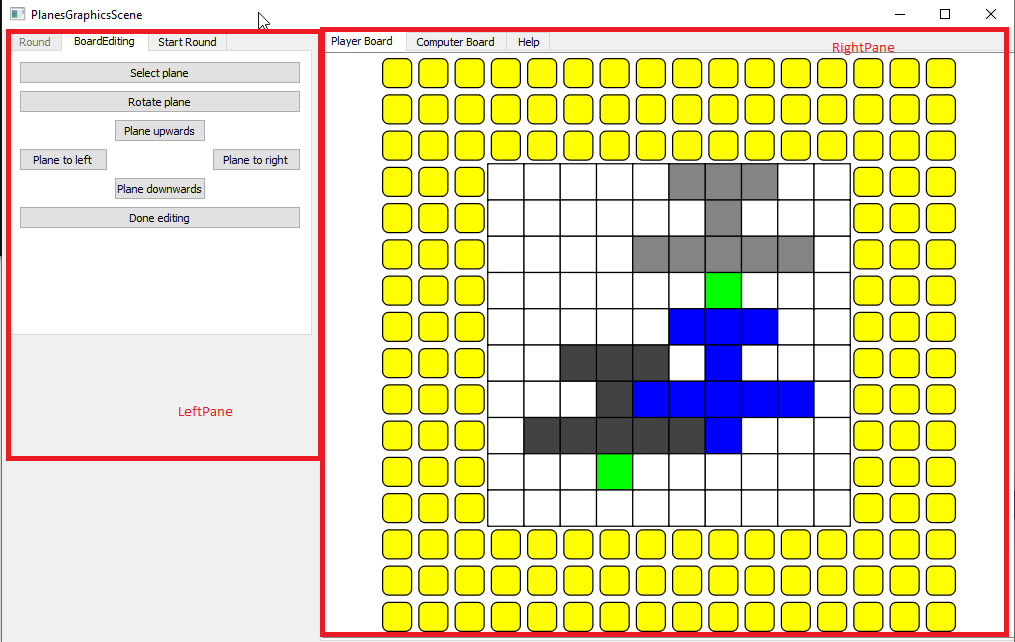
\includegraphics[width = \textwidth]{PlanesGraphicsScene_BoardEditing_WidgetNames.png}
	\caption{Simplified Layout of PlanesGraphicsScene}
	\label{fig:planesgraphicsscene_boardediting_widgetnames}
\end{figure}

The member variables for the PlanesGSView are:

\begin{lstlisting}

	//PlaneGrid objects manage the logic of a set of planes on a grid
	//as well as various operations: save, remove, search, etc.
	PlaneGrid* m_playerGrid;
	PlaneGrid* m_computerGrid;
	
	//PlaneRound is the object that coordinates the game
	PlaneRound* m_round;
	
	LeftPane* m_LeftPane;
	RightPane* m_RightPane;

\end{lstlisting}

Better as in the PlanesWidget project, the ComputerLogic object is not extracted from the PlaneRound anymore, only the two PlaneGrid objects are, which is still not satisfactory. The widgets composing the GUI are grouped under two principal widgets: LeftPane and RightPane.

The layout of the PlanesGSView is defined as follows:

\begin{lstlisting}
	CustomHorizLayout* hLayout = new CustomHorizLayout(this);
	m_LeftPane = new LeftPane(this);
	m_LeftPane->setMinWidth();
	//m_LeftPane->setSizePolicy(QSizePolicy::Fixed, QSizePolicy::Expanding);
	
	m_RightPane = new RightPane(*m_playerGrid, *m_computerGrid, this);
	m_RightPane->setMinWidth();
	
	hLayout->addWidget(m_LeftPane);
	hLayout->addWidget(m_RightPane);
	setLayout(hLayout);
\end{lstlisting} 

In principle it is a customized horizontal layout (see \ref{custom_qt_layout}) containing the LeftPane and RightPane widgets (see Figure \ref{fig:planesgraphicsscene_boardediting_widgetnames}). 

\subsection{LeftPane}
The LeftPane widget is a QTabWidget, a widget displaying more tabs. There is one tab for each game stage. To each of these tabs corresponds one widget: m\_BoardEditingWidget, m\_GameWidget, m\_StartGameWidget.

The class defines methods to interact when a new game stage starts:

\begin{lstlisting}
    void activateGameTab();
	void activateEditorTab();
	void activateStartGameTab();
\end{lstlisting}

It also defines signals that symbolize clicks on the different buttons in the interface:

\begin{lstlisting}
    void selectPlaneClicked(bool);
	void rotatePlaneClicked(bool);
	void upPlaneClicked(bool);
	void downPlaneClicked(bool);
	void leftPlaneClicked(bool);
	void rightPlaneClicked(bool);
	void doneClicked();
	void startNewGame();
\end{lstlisting}

Finally it defines how the widget reacts to external events, throught the following slots:

\begin{lstlisting}

	/**
	* @brief When planes overlap deactivate the done button
	* @param planesOverlap - received info from corresponding signal
	*/
	void activateDoneButton(bool planesOverlap);
	
	/**
	* @brief Activate the game tab when the done button is clicked
	*/
	void doneClickedSlot();
	
	/**
	* @brief activates the editing board tab and the buttons in it
	*/
	void activateEditingBoard();
	
	/**
	* @brief Updates the statistics in the left pane
	*/
	void updateGameStatistics(const GameStatistics& gs);
	
	/**
	* @brief
	* Hide the other tabs.
	*/
	void endRound(bool isPlayerWinner);

\end{lstlisting}

\subsection{RightPane}

The RightPane is a QTabWidget as well with 3 tabs: player's game board, computer's game board and the help page.

The RightPane emits two signals:

\begin{lstlisting}
	void planePositionNotValid(bool);
	void guessMade(const GuessPoint& gp);
\end{lstlisting}

and reacts to signals with the slots:

\begin{lstlisting}
    void resetGameBoard();
	void selectPlaneClicked(bool);
	void rotatePlaneClicked(bool);
	void upPlaneClicked(bool);
	void downPlaneClicked(bool);
	void leftPlaneClicked(bool);
	void rightPlaneClicked(bool);

	/**
	* @brief Switch to computer tab and start looking for planes.
	* Change the internal state of the player's and computer's boards to game stage
	*/
	void doneClicked();
	
	/**
	* @brief Display winner message in the player and computer boards.
	* Block mouse click events in the computer board.
	*/
	void endRound(bool isPlayerWinner);
	void startNewGame();
	void showComputerMove(const GuessPoint& gp);
\end{lstlisting}

The core of the RightPane class are the two game boards, implemented in the classes: PlayerBoard and ComputerBoard.

\subsection{The Game Boards}

Both PlayerBoard and ComputerBoard derive from the class GenericBoard, that provides the tools to interact with a PlaneGrid object from the game controller in order to display the planes and guesses throughout the game.

PlayerBoard and ComputerBoard in PlanesGraphicsScene correspond to GameRenderArea from the PlanesWidget. GenericBoard in PlanesGraphicsScene corresponds to BaseRenderArea in PlanesWidget.

The most important improvement brought by GenericBoard when compared to BaseRenderArea is that it is not a QWidget where the paintEvent() method was overriden, but it uses a specialized framework of Qt: the GraphicsScene/GraphicsView framework.

The display of the board works as follows: the GenericBoard class keeps a collection of GridSquare objects, one for each square of the game board. The GridSquare objects can be parts of the plane, empty squares, plane head, and guesses(hit, miss or dead). When the program is started GridSquare objects are created for every square on the player and computer game boards. Throughout the game, the GameBoard object reads the state of the game from the game engine (PlaneRound), and updates the GridSquare objects accordingly.

\subsection{Qt Concepts}

\subsubsection{Implementing a Custom Layout} \label{custom_qt_layout}

A custom layout was used for the PlanesGSView class:

\begin{lstlisting}
int CustomHorizLayout::count() const
{
	return m_ItemsList.size();
}

QLayoutItem* CustomHorizLayout::itemAt(int idx) const
{
	// QList::value() performs index checking, and returns 0 if we are
	// outside the valid range
	return m_ItemsList.value(idx);
}

QLayoutItem* CustomHorizLayout::takeAt(int idx)
{
	// QList::take does not do index checking
	return idx >= 0 && idx < m_ItemsList.size() ? m_ItemsList.takeAt(idx) : 0;
}

void CustomHorizLayout::addItem(QLayoutItem* item)
{
	if (count() < 2)
		m_ItemsList.append(item);
}

CustomHorizLayout::~CustomHorizLayout()
{
	QLayoutItem *item;
	while ((item = takeAt(0)))
	delete item;
}

void CustomHorizLayout::setGeometry(const QRect &r)
{
	QLayout::setGeometry(r);
	
	///only two widgets can lie in this layout
	if (count() != 2)
	return;
	
	QList<int> scalHoriz;
	
	scalHoriz.append(20);
	scalHoriz.append(80);
	
	int w = r.width() - (count() + 1) * spacing();
	int i = 0;
	int curX = 0;
	while (i < count()) {
		QLayoutItem *o = m_ItemsList.at(i);
		int wtemp = (w * scalHoriz[i]) / 100;
		int htemp = r.height();
		if (i == 0) {
			wtemp = std::max(wtemp, o->minimumSize().width());
			htemp = std::max(r.height() / 2, o->minimumSize().height());
		} else {
			wtemp = std::max(r.width() - curX - spacing(), o->minimumSize().width());
		}
		QRect geom(r.x() + curX + (i + 1) * spacing(), r.y(), wtemp, htemp);
		o->setGeometry(geom);
		++i;
		curX += wtemp;
	}
}

QSize CustomHorizLayout::sizeHint() const
{
	QSize s(0,0);
	int n = m_ItemsList.count();
	if (n > 0)
		s = QSize(1000, 600); //start with a nice default size
	int i = 0;
	while (i < n) {
		QLayoutItem *o = m_ItemsList.at(i);
		s = s.expandedTo(o->sizeHint());
		++i;
	}
	return s + n*QSize(spacing(), spacing());
}

QSize CustomHorizLayout::minimumSize() const
{
	QSize s(0,0);
	int n = m_ItemsList.count();
	int i = 0;
	while (i < n) {
		QLayoutItem *o = m_ItemsList.at(i);
		s = s.expandedTo(o->minimumSize());
		++i;
	}
	return s + n*QSize(spacing(), spacing());
}

\end{lstlisting}

The class CustomHorizLayout extends QLayout. It is a layout that accepts only two widgets, the condition is defined in the addItem() function. The most important function is setGeometry(). Here we define that given a total layout size w, the width of the LeftPane widget (the first to be added in the layout) is

\begin{lstlisting}
	std::max((w * 20) / 100;, o->minimumSize().width());
\end{lstlisting}

where o is the LeftPane widget, which has defined a minimumSize() based on the display size of strings that are to be displayed in the widget.

The RightPane should be displayed directly near the LeftPane with a width of 

\begin{lstlisting}
	std::max(r.width() - curX - spacing(), o->minimumSize().width());
\end{lstlisting}

That means it will take the remaining size width as long as this width is not smaller as the minimum width of the RightPane widget (which is defined in the minimumSize() function for the widget)

The other functions of the class are standard functions, like they are shown in tutorials on the Qt website.

\subsubsection {GraphicsScene - GraphicsView Framework of Qt}

The framework allows to create a space (or scene) (QGraphicsScene) where objects (QGraphicsItems) are displayed. The objects can be added to the scene with a addItem() function. During their lifetime objects can move on the scene, be deleted or change their appearance.

In PlanesGraphicsScene the graphic items objects are of the class GridSquare, which derives from QGraphicsItem, and in the derived class PlayAreaGridSquare. In order to define the appearance of the graphic objects one has to override the function paint() from the QGraphicsItem class.

For example in the PlayAreaGridSquare:

\begin{lstlisting}
void PlayAreaGridSquare::paint(QPainter* painter, const QStyleOptionGraphicsItem* option, QWidget* widget) {
	Q_UNUSED(option)
	Q_UNUSED(widget)
	
	painter->setRenderHint(QPainter::Antialiasing);
	drawCommonGraphics(painter);
	
	if (m_ShowGuesses) {
		switch(m_Status) {
		case GameStatus::Empty:
		break;
		case GameStatus::PlaneGuessed:
		drawPlaneGuessed(painter);
		break;
		case GameStatus::PlaneHeadGuessed:
		drawPlaneHeadGuessed(painter);
		break;
		case GameStatus::TestedNotPlane:
		drawTestedNotPlane(painter);
		break;
		}
	}
}

void PlayAreaGridSquare::drawCommonGraphics(QPainter* painter)
{
	if (m_Selected) {
		painter->fillRect(boundingRect(), Qt::blue);
	} else {
		if (m_ShowPlane) {
			switch(m_Type) {
			case Type::Empty:
			painter->fillRect(boundingRect(), Qt::white);
			break;
			case Type::PlaneHead:
			painter->fillRect(boundingRect(), Qt::green);
			break;
			case Type::Plane:
			painter->fillRect(boundingRect(), m_Color);
			break;
			}
		} else {
			painter->fillRect(boundingRect(), Qt::white);
		}
	}
	
	//    if ((m_ShowPlane && m_Type != Type::Empty) || m_Selected)
	//        painter->setPen(Qt::magenta);
	//    else
	painter->setPen(Qt::black);
	painter->drawRect(boundingRect());
}

void PlayAreaGridSquare::drawPlaneGuessed(QPainter* painter)
{
	QPainterPath fillPath;
	fillPath.moveTo(0, m_Width / 2);
	fillPath.lineTo(m_Width / 2, 0);
	fillPath.lineTo(m_Width, m_Width / 2);
	fillPath.lineTo(m_Width / 2, m_Width);
	fillPath.lineTo(0, m_Width / 2);
	painter->fillPath(fillPath, Qt::darkRed);
}

void PlayAreaGridSquare::drawPlaneHeadGuessed(QPainter* painter)
{
	painter->setPen(Qt::red);
	painter->drawLine(0, 0, m_Width, m_Width);
	painter->drawLine(0, m_Width, m_Width, 0);
}

void PlayAreaGridSquare::drawTestedNotPlane(QPainter* painter)
{
	QPainterPath fillPath;
	fillPath.addEllipse(m_Width / 4, m_Width / 4, m_Width / 2, m_Width / 2);
	painter->fillPath(fillPath, Qt::red);
}

\end{lstlisting}
\section {PlanesWidget}

\subsection{MainWindow}

The GUI is hosted by a QMainWindow of the derived class PlanesWWindow. The constructor of PlanesWWindow creates the game controller (a PlaneRound object) and gives it as parameter to the central area of the QMainWindow, which is an object of the class PlanesWView.


\begin{lstlisting}
PlanesWWindow::PlanesWWindow(QWidget *parent) :
	QMainWindow(parent)
{
	//builds the game object - the controller
	mRound = new PlaneRound(10, 10, 3);
	
	//builds the view object
	mPlanesView = new PlanesWView(mRound);
	setCentralWidget(mPlanesView);
	
	//starts the game
	mRound->initRound();
}

\end{lstlisting}

PlanesWView creates in the constructor the layout of the GUI. In Figure \ref{fig:planeswidget_game_widgetnames} are shown the names of the widgets used in the game area layout.

\begin{figure}[h]
	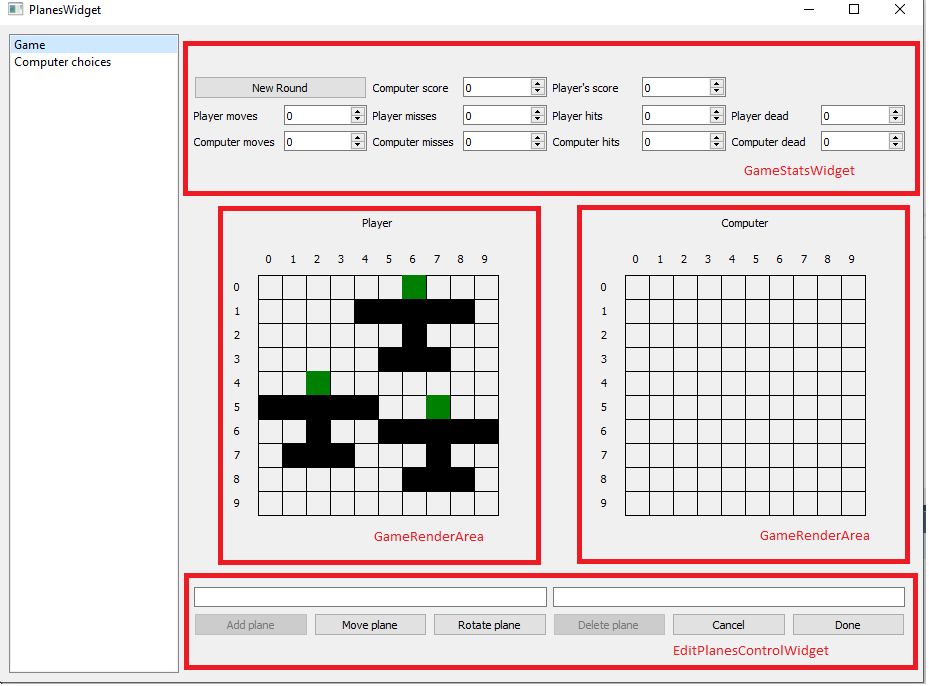
\includegraphics[width = \textwidth]{PlanesWidget_Game_WidgetNames.png}
	\caption{Widgets in the game area layout}
	\label{fig:planeswidget_game_widgetnames}
\end{figure}

\subsection {Qt Concepts}

\subsubsection {QMainWindow}
\subsubsection {QWidget}

\end{document}